%%%%%%%%%%%%%%%%%%%%%%%%%%%%%%%%%%%%%%%%%%%%%%%%%%%%%%%%%%%%%%%
%
% Welcome to writeLaTeX --- just edit your LaTeX on the left,
% and we'll compile it for you on the right. If you give 
% someone the link to this page, they can edit at the same
% time. See the help menu above for more info. Enjoy!
%
%%%%%%%%%%%%%%%%%%%%%%%%%%%%%%%%%%%%%%%%%%%%%%%%%%%%%%%%%%%%%%%
%
% For more detailed article preparation guidelines, please see:
% http://f1000research.com/author-guidelines

\documentclass[10pt,a4paper,twocolumn]{article}
\usepackage{f1000_styles}
\usepackage{url}
\usepackage{tabularx}
\bibliographystyle{f1000}

\newcommand{\tick}{\mbox{$\surd$}}


\begin{document}

\title{Viewing multiple sequence alignments with
  the {J}avaScript {S}equence {A}lignment {V}iewer (JSAV)}

\author[1]{Andrew C. R. Martin}
\affil[1]{andrew@bioinf.org.uk -or- andrew.martin@ucl.ac.uk \\
  Corresponding author\\
  Institute of Structural and Molecular Biology,\\
  Division of Biosciences, University College London,\\
  Darwin Building, Gower Street,\\
  London WC1E 6BT}

\maketitle

\begin{abstract}

The JavaScript Sequence Alignment Viewer (JSAV) is designed as a simple-to-use JavaScript component for displaying sequence alignments on web pages.  The display of sequences
is highly configurable with options to allow alternative colouring
schemes, sorting of sequences and `dotifying' repeated amino acids. An
option is also available to submit selected sequences to another web
site, or to other JavaScript code. 
JSAV is implemented purely in JavaScript making use of the JQuery and
JQuery-UI libraries. It does not use any HTML5-specific options to help with
browser compatibility. The code is documented using JSDOC
and is available from \url{http://www.bioinf.org.uk/software/jsav/}

\end{abstract}
\listoftodos[F1000Research review comments] % Ignore until review stage
\clearpage

%%%%%%%%%%%%%%%%%%%%%%%%%%%%%%%%%%%%%%%%%%%%%%%%%%%%%%%%%%%%%%%%%%%%
\section*{Introduction}
Viewing multiple sequence alignments (MSAs) is a fundamental
requirement in analysis of protein sequences, allowing us to visualize
conservation across protein families as well as unusual features of
particular sequences. As a result, there are a plethora of tools for
viewing MSAs. These range from tools which provide attractive printed
output, through standalone graphical tools --- either operating-system
dependent, or independent --- to web-based viewers.

Two of the earliest tools were HOMED\cite{stockwell:homed} and
MALIGNED\cite{clark:maligned} written for VAX/VMS workstations.
Neither seems to be actively maintained or easily available any
more. Other early viewers include GeneDoc\cite{nicholas:genedoc},
BioEdit, Seaview\cite{galtier:seaview} and DCSE\cite{derijk:dcse}
which is part of the RnaViz package for visualizing RNA secondary
structure\cite{derijk:rnaviz}, but which can be used for protein
sequence alignments.  A problem in writing graphical software is the
operating-system dependency of many graphics libraries.
CINEMA\cite{parrysmith:cinema} was probably the first sequence
alignment viewer and editor implemented in Java, a platform
independent programming language allowing graphical user interfaces
(GUIs) to run on any operating system. It has now been rewritten in
C++ and is part of UTOPIA\cite{pettifer:utopia}. Other software
includes MPSA\cite{blanchet:mpsa}, ANTHEPROT\cite{deleage:antheprot}
and ClustalX\cite{thompson:clustalx}, a GUI for the ClustalW multiple
sequence alignment program, providing an integrated environment for
aligning sequences and analyzing results. Clustal Omega is the most
recent version, but at the time of writing only has a command line
interface --- a beta version of a GUI is due to be released soon.

More recent developments include the Protein Family Alignment
Annotation Tool (PFAAT)\cite{johnson:pfaat} designed specifically for
family analysis and incorporating residue annotation tools as well as
integration with Jmol for protein structure display. Like early
versions of CINEMA, PFAAT is implemented in Java for operating system
independence. CLC~Viewer is a recent free package written in Java
which contains a number of integrated tools and acts as a core product
for adding other features through a commercial version.  A more
complete list of MSA viewers is available on the web at
\url{http://en.wikipedia.org/wiki/List_of_alignment_visualization_software}.

Probably the most popular of the available tools is
Jalview\cite{clamp:jalview} which is available in two versions: a
standalone Java application which provides many tools and facilities,
and as a `light' version (JalviewLight) --- a Java applet that can be
embedded in a web page. The latter responds to the need for web site
developers to be able to embed MSA visualization.

However, in recent years there has been a gradual move away from using
Java applets in web development.  Java creates an additional layer of
software (including additional memory consumption) and modern browsers
enforce much more caution in running Java applets to avoid security
threats. This can result in user irritation with having to accept
various popup warnings and/or configure security settings, often
having to repeat this process when there is a software update. It is
not uncommon for Java applets simply to fail to run, perhaps because
users do not understand what settings need to be changed.  New HTML
features such as the HTML5 Canvas, and powerful JavaScript libraries
such as Bootstrap, JQuery and JQuery-UI that provide an easier syntax
for accessing elements of a web page together with new widgets such as
sliders and drag-and-drop support, have overtaken Java as the method
of choice for creating interactive web sites with complex
requirements.  Such features are used widely by popular web sites such
as Google Mail, Google Docs, Twitter and Facebook.  Illustrating this
trend, the Jmol structure viewer has recently been reimplemented in
JavaScript as JSmol (\url{http://sourceforge.net/projects/jsmol/}).

Consequently, over the last couple of years a small number of
JavaScript-based sequence and alignment viewers have started to be
developed. These include MODalign\cite{barbato:modalign},
Alignment-Annotator\cite{gille:2014aa}, SnipViz\cite{jaschob:2014},
and Sequence\cite{gomez:2014}, a component of the BioJS
library\cite{corpas:biojs}. In addition, there is an intention to port
JalviewLight to JavaScript.  The available programs are briefly
reviewed:

\begin{figure*}[t]
%\footnotesize
\begin{verbatim}
var MySeqs = Array();
MySeqs.push({ id :"id1b1.L", sequence :"SASSSVNYMYACREFGHIKLMNPTRSTVWY"});
MySeqs.push({ id :"id1a.L",  sequence :"SASSSTNYMYACDEFGHIKLMNPQRSTVWY"});
MySeqs.push({ id :"id2b1.L", sequence :"SASSTCNYMTACDEEGHIKLMNP-RSTCWY"});

var MyOptions = Array();
MyOptions.sortable = true;
MyOptions.selectable = true;
MyOptions.deletable = true;
MyOptions.toggleDotify = true;
MyOptions.toggleNocolour = true;
MyOptions.consensus = true;
MyOptions.selectColour = true;

printJSAV('sequenceDisplay', MySeqs, MyOptions);
\end{verbatim}
\caption{\label{fig:code}Example code illustrating the creation of a
JavaScript array of sequence objects, the options and the call
necessary to create the alignment viewer.}
\end{figure*}


\begin{description}
\item[MODalign] is part of the MODexplorer
  package\cite{kosinski:2013}, a web site for protein modelling, but
  does not appear to be available as a download for use in other web
  sites.
\item[Alignment-Editor] is part of a more complex system, STRAP. It
  uses a Java server-side interpreter,
  Alignment-to-HTML\cite{gille:2014}, which parses the STRAP scripting
  language and creates an alignment in a form that can be rendered in
  Web browsers. The server-side element allows tasks such as sequence
  retrieval, computation of alignments and communication with
  BioDAS-servers. The rendering system includes a selection of
  colouring schemes, highlighting of conserved and variable positions
  in the alignment, reordering and deletion of sequence by
  drag-and-drop, and residue annotation as well as links to 3D
  visualization and sequence groups. It exploits JavaScript and HTML5
  using the HTML5 canvas to draw helices and other visual elements.
  However the JavaScript visualizer does not appear to be available by
  itself. The description of Alignment-Editor\cite{gille:2014aa}
  suggests that alignments should be prepared using the full Java
  system and the final alignment can then be downloaded as HTML files
  in a ZIP archive. The software is licensed under the GPL and
  available from the authors on request, or a desktop version of STRAP
  can be downloaded or run using Java WebStart. While in principle
  possible, no simple documentation is provided to enable the
  client-side JavaScript/HTML5 viewer to be used without the server
  side software.
\item[SnipViz] is a compact and lightweight component designed for
  display of multiple versions of gene and protein sequences --- i.e.\
  essentially identical sequences with mutations.  It provides a very
  simple clean display focused around both DNA and protein sequences
  allowing very long sequences through a scrolling mechanism which
  also shows a small box on a representation of the complete sequence
  to show the relative position within the complete alignment.  It
  also allows display of phylogenetic trees stored in Newick
  format. Note that SnipViz should not be confused with
  SNPViz\cite{langewisch:snpviz}.
\item[Sequence] is a BioJS component for visualizing sequences rather
  than alignments.  It only provides very simple views with no choices
  of colouring schemes, although it does provide very flexible
  highlighting of regions within a sequence.
\end{description}

\begin{table*}
\footnotesize
\begin{center}
\begin{tabularx}{\linewidth}{Xlllll} \hline
                                  &       & MOD-     & Alignment-       &         &          \\
                                  & JSAV  &    align &           Editor & SnipViz & Sequence \\ \hline
Simple, lightweight component     & \tick & \dag     & \ddag            & \tick   & \tick    \\
Flexible colouring schemes        & \tick & \tick    & \tick            &         &          \\
Dotifying                         & \tick &          &                  &         &          \\
Automatic sequence sorting        & \tick &          &                  &         &          \\
Manual sequence sorting           &       &          & \tick            &         &          \\
Remove sequences                  & \tick &          & \tick            &         &          \\
Highlight regions                 & \tick &          & \tick            & \S      & \tick    \\
FASTA export                      & \tick & \tick    & \tick            &         & \tick    \\
Submission to another site        & \tick & *        &                  &         &          \\
Submission to JavaScript          & \tick &          &                  &         &          \\
Display consensus sequence        & \tick & \tick    & \P               &         &          \\
Display secondary structure       &       & \tick    & \tick            &         &          \\
Alignment editing                 &       & \tick    &                  &         &          \\
Link to structure viewer          &       & \tick    & \tick            &         &          \\
Display phylogenetic tree         &       &          &                  & \tick   &          \\
Optimized for very long sequences &       &          &                  & \tick   &          \\ \hline
\end{tabularx}
\end{center}
\caption{\label{tab:features}Summary of availability of features in
  various JavaScript sequence alignment display tools as described in
  their respective papers and web sites. Note that the MODAlign web
  site was unavailable at the time of writing so capabilities have
  been judged purely on what is published in the paper. \dag~not
  available for use in other web sites. \ddag~Should be possible,
  but not designed to be used in this way. *~Submission to Modeller
  only. \S~Automatically highlights mutated residues. \P~highlights
  columns of residues conserved at a specified level rather than
  displaying a consensus.} 
\end{table*}

JSAV (JavaScript Sequence Alignment Viewer) is a novel JavaScript
component that adds to this list. The primary motivation for
implementing a new tool was for development of our abYsis antibody
database (\url{http://www.abysis.org/}), where we required a simple
JavaScript component that would enable us to display a set of aligned
sequences, sort and select sequences in that alignment for further
analysis, and highlight regions of the alignment corresponding to the
CDR loop regions of antibodies. Consequently the requirements were as
follows: (i)~a very simple-to-use lightweight component that can
easily be dropped into a web site; (ii)~provision of flexible
colouring schemes and `dotifying' alignments (replacing repeated
residues with dots); (iii)~the ability to sort sequences --- based
both on complete sequences or regions of sequences (such as a CDR loop
or framework region of an antibody); (iii)~the ability to remove
sequences from the alignment; (iv)~the ability to highlight regions in
the alignment and to display a consensus sequence; (v)~the ability to
export a selected set of sequences in FASTA format; (vi)~the ability
to submit a selected set of sequences to another web site or to
client-side JavaScript code for further processing.
Table~\ref{tab:features} lists the availability of these and other
features in different tools.

%%%%%%%%%%%%%%%%%%%%%%%%%%%%%%%%%%%%%%%%%%%%%%%%%%%%%%%%%%%%%%%%%%%%
\section*{Software tool}


\begin{figure}
\centering
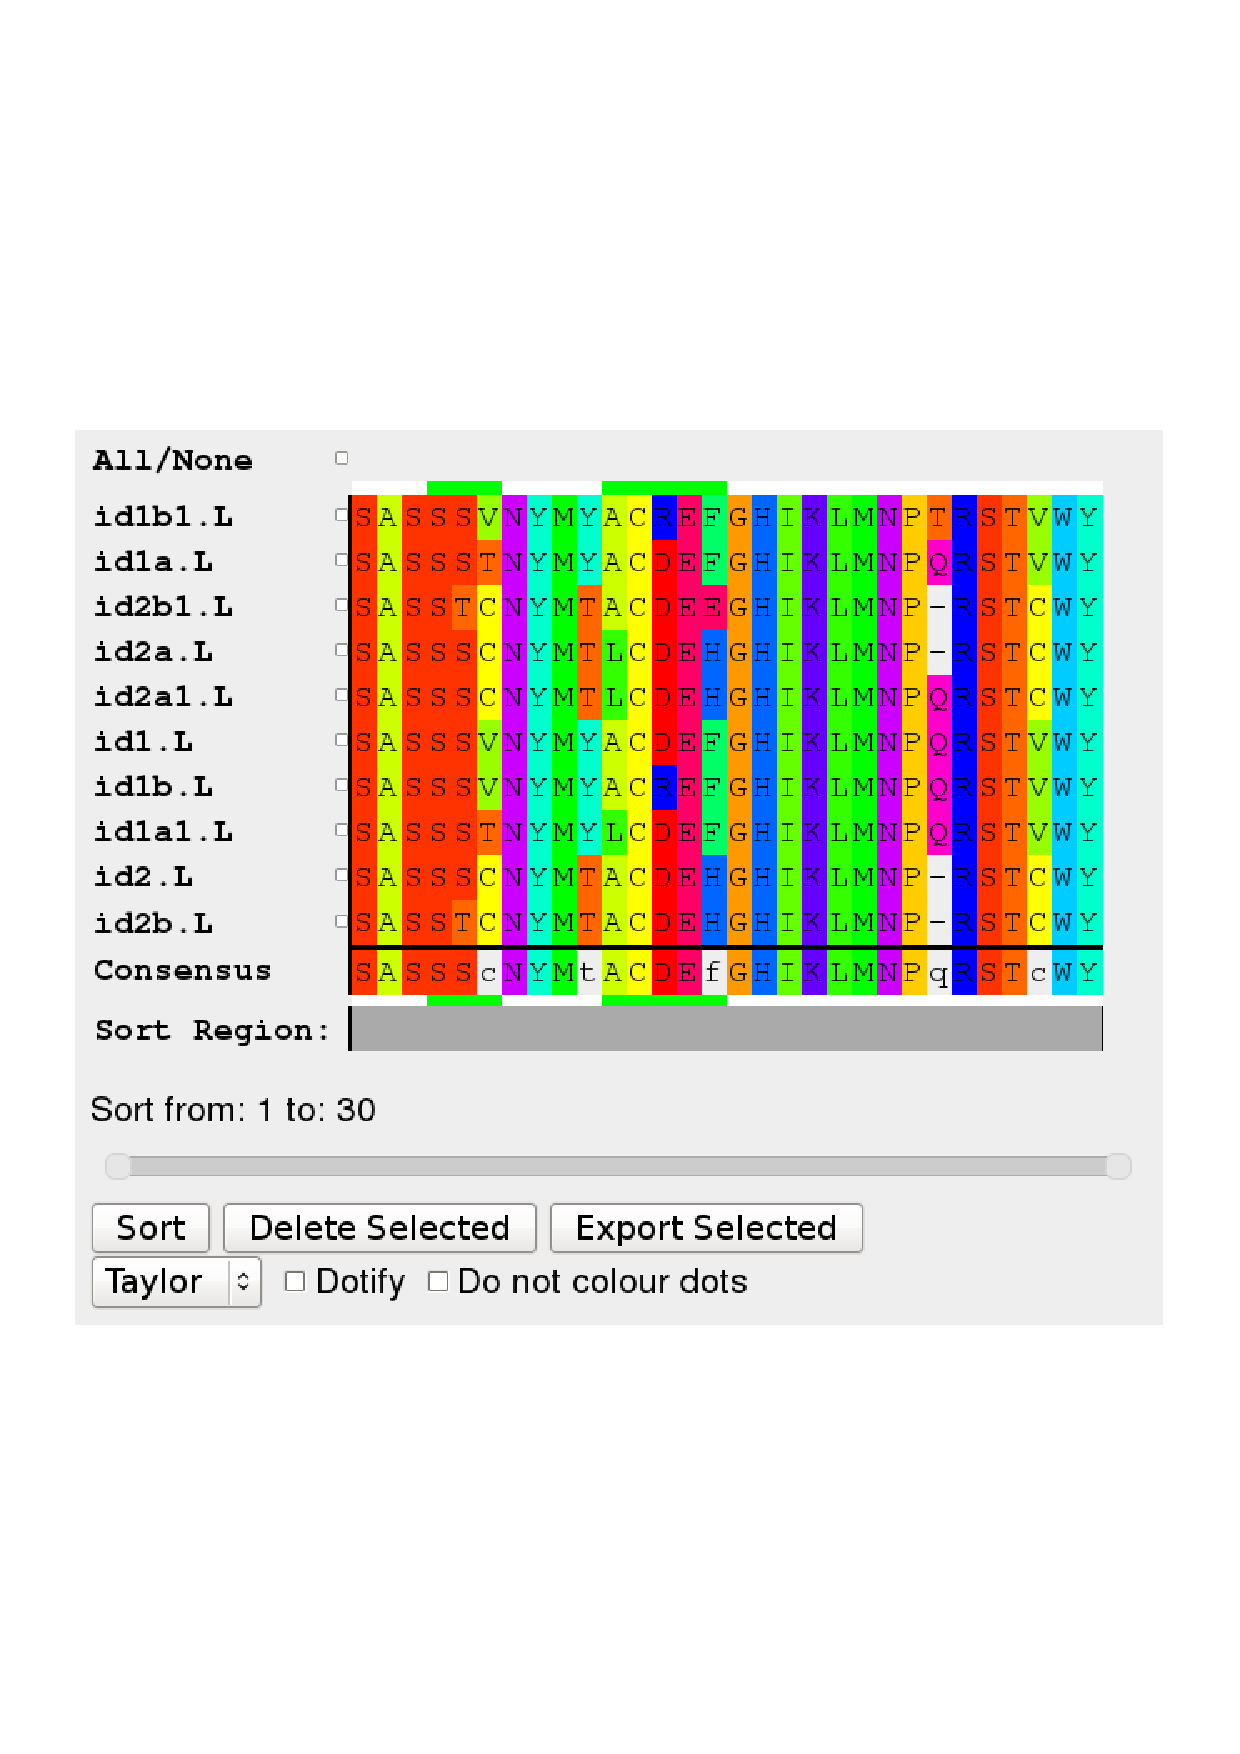
\includegraphics[width=\columnwidth]{demo.png}
%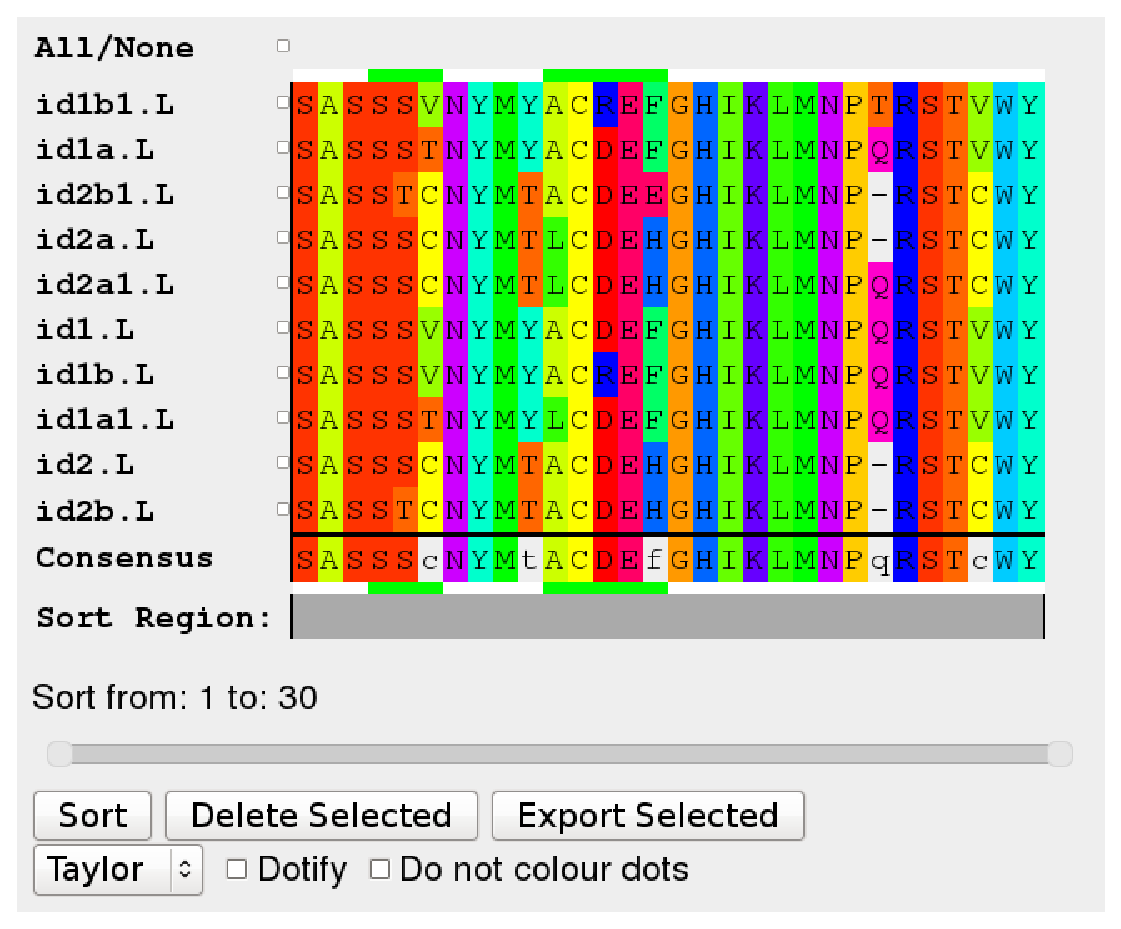
\epsfig{file=demo.eps,width=\columnwidth}
\caption{\label{fig:demo}A typical JSAV alignment view}
\end{figure}

JSAV allows the end-user to modify the display in a number of ways.
The web-site provider has control over which of these is available to
the end user. First, the sequences can be sorted --- the code selects
the most representative sequence, displaying that at the top of the
alignment followed by the most similar sequence and so on. By default,
sorting is performed across the whole sequence, but a two-handled
slider allows the range of positions on which the sort is based to be
modified. Different colouring schemes are available duplicating those
provided in Jalview. The alignment can also be `dotified', replacing
residues repeated between sequences with dots in order to emphasize
amino acid differences. Colouring of dotified residues can also be
switched off or on. Sequences can be selected and deleted from the
alignment; a consensus sequence can be displayed at the bottom of the
alignment and updates automatically when sequences are deleted. The
complete set of sequences, or a selected subset, can be submitted to
another web site, or passed to another JavaScript function for
integration with other tools. Tooltips are provided for each option
and all options are documented in detail on the web site.

JSAV is implemented purely in JavaScript. Code is managed using GitHub
(\url{http://www.github.com}) and documented using JSDOC
(\url{http://usejsdoc.org}). JSAV employs the JQuery library to ease
access to elements of the HTML that it generates and uses JQuery-UI to
implement a two-value slider that is used to specify a range of
positions in the alignment.  As input, the code requires an array of
JavaScript objects which contain two elements: a unique identifier for
a sequence and the sequence itself --- all sequences must be
pre-aligned.  Secondly a set of options can be provided. Options fall
into two classes - those that control the (initial) display and those
that control facilities available to the end user of a web site to
modify the view of the MSA. Options that control the display include:
(i)~ranges of alignment column positions to be highlighted; (ii)~the
colour scheme to be used; (iii)~whether the sequence should be
dotified and whether repeated residues should be coloured;
(iv)~whether a consensus sequence should be displayed; (v)~whether a
FASTA export button should be available and the label for that button;
(vi)~the URL and label for a button to allow selected sequences to be
submitted to another web site; (vii)~a JavaScript function name and
label for a button to allow selected sequences to be processed by code
written by the web site developer; (viii)~whether plain tool tips
should be used rather than those provided by JQuery --- more
attractive tooltips available with the `tooltipster' package are also
supported. Options that control how the end-user can manipulate the
display include: (i)~whether the alignment should be sortable and, if
so, the width and height of the slider used to select a region for
sorting (ii)~whether selection checkboxes should be displayed next to
each sequence (iii)~whether sequences can be deleted from the
alignment (iv)~whether the user should be able to toggle the dotifying
of the alignment (v)~whether the user should be able to toggle not
colouring dotified residues (vi)~whether a pull-down should be
displayed to select colour schemes.

The sequence alignment is rendered as a table and all display of
colours and layout is achieved through Cascading Style Sheets (CSS).
Consequently a web-site developer can easily add a new colour scheme
by modifying the CSS file and setting an option to specify available
colour scheme names.  The number and size of sequences in the MSA is
limited only by the memory available to the web browser.  A brief
extract of sample code is shown in Figure~\ref{fig:code} with the
results shown in Figure~\ref{fig:demo}.

JSAV deliberately avoids making use of HTML5 to maximize browser
compatibility. It is known to work with modern browsers including
Firefox~V32.0, Chrome~V37, Konqueror~V4.13.3, Safari~V5.1.7 and
Explorer~V10.0 on Linux, Mac and Windows platforms and is known to
work on versions of Firefox as old as V9.0.1. JSAV has been developed
and tested using JQuery V1.10.2 and JQuery-UI V1.10.4, but it only
uses the JQuery HTML element selection mechanism and tool tips and the
two-handled slider component from JQuery-UI and consequently would be
expected to work with much earlier versions.

%%%%%%%%%%%%%%%%%%%%%%%%%%%%%%%%%%%%%%%%%%%%%%%%%%%%%%%%%%%%%%%%%%%%
\section*{Conclusions}
Viewing multiple sequence alignments is a fundamental requirement of
protein sequence analysis. With that large amounts of Bioinformatics
work being performed over the web, there is a clear need to be able to
embed MSA viewers within web pages. The recent move away from Java in
favour of JavaScript has driven a need for MSA viewing tools written
in JavaScript. While four other tools have been made available, two do
not appear to be available as simple components that can be used by a
web developer to provide sequence alignments (MODalign and
Alignment-Editor). Of the other two, SnipViz has only very limited
facilities and is designed for viewing SNPs in alignments of very
similar sequences while Sequence is only designed for displaying single
sequences not MSA.

Consequently JSAV fills this gap, providing a very simple-to-use
component that can just be passed an array or pre-aligned sequences,
but which also has the flexibility to allow manipulation of the way in
which the MSA is displayed. JSAV provides a number of features that
appear to be absent from any of the other tools including dotifying
alignments, automatic sorting of sequences (including limiting the
sort to a region within the MSA), and submission of selected sequences
to other web sites or to other JavaScript code.

Future directions are likely to include modifying the JSAV component
to become part of BioJS\cite{corpas:biojs} and linking JSAV with JSMol
for structure visualization.


%%%%%%%%%%%%%%%%%%%%%%%%%%%%%%%%%%%%%%%%%%%%%%%%%%%%%%%%%%%%%%%%%%%%
\section*{Software availability}
The software is licensed under the GPL and may be downloaded from
\url{http://www.bioinf.org.uk/software/jsav/} where demonstrations,
including the ability to upload your own MSA, are available together
with full documentation implemented with JSDOC. The software is managed on GitHub at \url{http://www.github.com/AndrewCRMartin/JSAV}.

%%%%%%%%%%%%%%%%%%%%%%%%%%%%%%%%%%%%%%%%%%%%%%%%%%%%%%%%%%%%%%%%%%%%
\section*{Competing interests}
JSAV was developed under a grant for commercialization of abYsis, a web-based antibody database and analysis platform (\url{http://www.abysis.org/}. JSAV is used as part of abYsis in which University College London and the author have a financial interest.

%%%%%%%%%%%%%%%%%%%%%%%%%%%%%%%%%%%%%%%%%%%%%%%%%%%%%%%%%%%%%%%%%%%%
\section*{Grant information}
Development of this software was funded as part of a BBSRC Follow-On
grant (BB/K015443/1).

%%%%%%%%%%%%%%%%%%%%%%%%%%%%%%%%%%%%%%%%%%%%%%%%%%%%%%%%%%%%%%%%%%%%
\section*{Acknowledgements}
ACRM thanks the UCL Research Software Development team (in particular,
Jens Nielsen) for their contributions to JSAV.

\bibliography{jsav}

\end{document}

